\documentclass{standalone}
\usepackage{tikz,bm}
\begin{document}

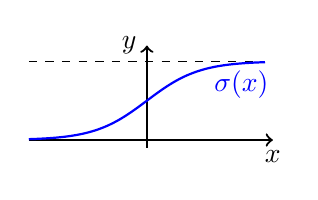
\begin{tikzpicture}

% Draw axes
\draw[thick,->] (-1.5,0) -- (1.6,0) node[anchor=north] {$x$};
\draw[thick,->] (0,-0.1) -- (0,1.2) node[anchor=east] {$y$};
\draw[dashed] (-1.5,1) -- (1.5,1);

% Draw sigmoid function
\draw[thick, domain=-1.5:1.5, smooth, variable=\x, blue] plot ({\x},{1/(1+exp(-3*\x))});

\node[blue] at (1.2, 0.7) {$\sigma(x)$};

\end{tikzpicture}

\end{document}
